\newlecture

\setcounter{section}{4}
%\def\textbookchapter{Chapter 9: Multivariable and Vector Functions}
\def\coursetopicnumber{I}
\def\textbooksection{9.5} % corresponding textbook section
\def\topic{Lines and Planes in Space} % this is the printed title
\def\shorttopic{Lines and planes} % short topic
\def\textbookname{Active Calculus} % this is the corresponding textbook
\def\textbooksectionurl{https://activecalculus.org/vector/S-9-5-Lines-Planes.html} % URL for textbook section
\def\handoutday{} % this is the printed date

%%%%%%%%% DOCUMENT CONTENT STARTS BELOW

\thispagestyle{plain}
\topstuff
\section{\topic{} \booklink{}}
\label{sec:lines-and-planes}

\subsection{Vector-valued functions}
In Definition~\ref{defn:position-vector}, we defined a \emph{position vector} as a vector that has its tail at the origin (denoted $O$). We'll often use the variable $\vec{r}$ to represent a position vector. If $P_0=(x_0,y_0,z_0)$ is a point in space, then the position vector that represents the point $P_0$ is $\vec{r}_0=\vec{OP_0}=\phantom{\vec{OP_0}=\langle x_0,y_0,z_0\rangle}$

\vspace{1.5in}

Since we are interested in position, we will typically work in $\mathbb{R}^2$ and $\mathbb{R}^3$. However, note that everything here applies in $\mathbb{R}^n$ for any $n\ge1$.

A vector in 3-space has the form $\vec{r}=\langle x,y,z\rangle$. If we want to introduce motion, we can take $x$, $y$, and $z$ to change over time. In other words, we make them functions of a new variable (often $t$).
\begin{defn}[Vector-valued function, parameter]
    A \emph{vector-valued function} is a function that takes one variable as input and outputs a vector (viewed as a position vector). In $\mathbb{R}^2$ and $\mathbb{R}^3$ a vector-valued function takes the form \medskip 
    \[
    \vec{r}(t)=\phantom{\langle x(t), y(t)\rangle} \hspace{1.6in} \text{ or } \quad \vec{r}(t)=\phantom{\langle x(t),y(t), z(t)\rangle,}\hspace{1.5in}\mbox{}
    \]
    \medskip 
    \\
    for $x(t)$, $y(t)$, $z(t)$ functions of $t$, with $t$ taking values from some interval. We call $t$ a \emph{parameter}. 
\end{defn}
The idea is that as the parameter $t$ changes, we get different position vectors that trace out a \emph{curve} (or path). For this reason, we call a vector-valued function a \emph{parametrization}.

We also say the functions $x(t)$, $y(t)$, $z(t)$ \emph{parametrize} the curve and we have \emph{parametric equations} written as 
\[
    \phantom{x=x(t),\quad y=y(t),\quad z=z(t).}
\]

\pagebreak 

\subsection{Lines in space}
We'll focus on lines here. (More general parametrizations are in Section \ref{sec:vector-valued-functions}.) When we sketch a vector-valued function, instead of drawing vectors, we just draw vector endpoints.

\begin{ex}
    Sketch $\vec{r}(t)=\langle 2,t\rangle$ for $t$ in $[0,3]$.
\end{ex}

\vfill 

\begin{ex}
    Sketch $\vec{r}(t)=\langle t,2\rangle$ for $t$ in $(-\infty,\infty)$.
\end{ex}

\vfill

\noindent Notice that any line can be described with a starting point and a direction!
\medskip

\begin{ex}
    Draw the line which goes through the point $P=(1,-1)$ with direction vector $\vec{v}=\langle 3,2\rangle$. Then draw the line which goes through the point $Q=(3,0)$ with direction vector $\vec{w}=\langle -2,1\rangle$.
\end{ex}
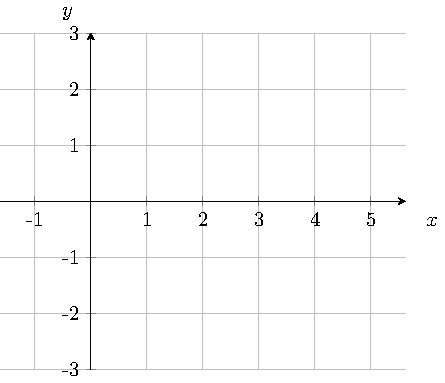
\includegraphics[scale=.8]{tikz-pictures/section-9.2-pic1-axes-for-vectors.pdf} 
\hfill 
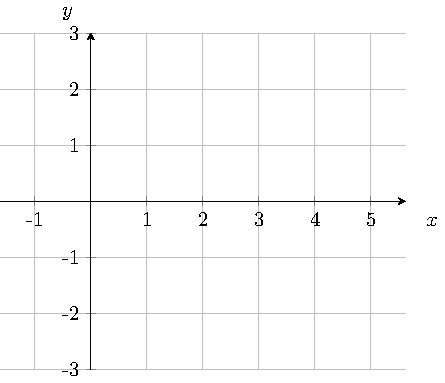
\includegraphics[scale=.8]{tikz-pictures/section-9.2-pic1-axes-for-vectors.pdf}

\begin{framed}
    \begin{thm}[Parametrization of a line]\label{thm:line-param}
        The line through the point $P_0$ (which has corresponding position vector $\vec{r}_0$) in the direction of the vector $\vec{v}$ is parametrized by the vector-valued function
        \[
            \vec{r}(t)=\hspace{.5in}\phantom{\vec{r}_0 + t\vec{v}\quad\quad,} \quad\quad\quad \quad \text{ for $t$ in \phantom{$(-\infty,\infty)$.}}
        \]
        If $\vec{r}_0=\langle x_0,y_0,z_0\rangle$ and $\vec{v}=\langle a,b,c\rangle$, then the parametric equations for this line are 
        \[
            x=\phantom{x_0+at,}\hspace{.3in} \ \quad \quad
            y=\phantom{y_0+bt,}\hspace{.3in} \quad \quad
            z=\phantom{z_0+ct,}\hspace{.3in} \quad \quad \text{ for $t$ in }\phantom{(-\infty,\infty).}
        \]
    \end{thm}
\end{framed}
\pagebreak

Note: To parametrize a line, we need a position vector (for a point on the line) and a direction vector. Since any line contains infinitely many points, and since we can scale the direction vector by any nonzero amount, any line has many different parametrizations!
\begin{ex}
    Find a vector-valued function that describes the line which goes through the points $P=(-1,4)$ and $Q=(3,-7)$. What are the corresponding parametric equations?
\end{ex}

\vfill

\begin{ex}
    Parametrize the line through the point $P=(2,3)$ with slope $-4$.
\end{ex}

\vfill

\begin{ex}
    Parametrize the line in $\mathbb{R}^3$ that goes through the $y$-axis at $y=3$ and through the $z$-axis at $z=-1$.
\end{ex}

\vfill

\pagebreak 

\subsection{Line segments}
In general, the vector-valued function $\vec{r}(t)=\vec{r}_0+t\vec{v}=\langle x_0+at, y_0+bt, z_0+ct\rangle$ with $t$ in the interval $(-\infty,\infty)$ describes a line which extends forever in both directions. If we want to describe just a segment of it, we can restrict the interval of $t$ values.
\begin{ex}
    Consider the vector-valued function $\vec{r}(t)=\langle 3+2t,-t,4\rangle$ with $t$ in the interval $[0,1]$. Describe this line segment. Where does it start and end?
\end{ex}

\vfill

\begin{ex}
    For $P=(1,2,3)$ and $Q=(-2,1,4)$, parametrize the line segment from $P$ to $Q$.
\end{ex}

\vfill\vspace{1.5in}

\begin{thm}[Line segment parametrization]
    In general, the line segment which starts at $P$ and ends at $Q$ is parametrized by
\end{thm}

\vspace{.7in}

\pagebreak

\subsection{Planes in \texorpdfstring{$\mathbb{R}^3$}{3-space}}
Our descriptions of lines can occur in $\mathbb{R}^n$ for any $n$. Now we focus on planes in $\mathbb{R}^3$.
%Just as we described lines in $\mathbb{R}^2$, we can describe planes in $\mathbb{R}^3$.
\begin{ex}
    Consider the plane that contains the point $P=(4,5,6)$ and that is orthogonal to the vector $\vec{n}=\langle 1,2,3\rangle$. If $Q=(x,y,z)$ is in the plane, find an equation that $Q$ satisfies.
\end{ex}

\vfill \vspace{.8in}

In general, if we have a point $P=(x_0,y_0,z_0)$ and a vector $\vec{n}=\langle a,b,c\rangle$, we can draw a plane through $P$ orthogonal to $\vec{n}$. A point $Q=(x,y,z)$ is in the plane precisely when $\vec{n}\dotp\vec{PQ}=0$.

Since $\vec{PQ}=\langle x-x_0,y-y_0,z-z_0\rangle$, we can rewrite this equation as \[\vec{n}\dotp\vec{PQ}=\hspace{5in}\]

\vfill

\begin{framed}
    \begin{thm}[Equation of a plane]
        Given any point $P=(x_0,y_0,z_0)$ and any nonzero vector $\vec{n}=\langle a,b,c\rangle$, the plane in $\mathbb{R}^3$ through $P$ orthogonal to $\vec{n}$ (called a \emph{normal vector}) is described by the equation
        \[
            \phantom{a(x-x_0)+b(y-y_0)+c(z-z_0)=0.}
        \] 
        Alternatively, we can write this as 
        \[
            \phantom{ax+by+cz=d, \text{\quad  where $d=ax_0+by_0+cz_0$}.}
        \]
    \end{thm}
\end{framed}
\begin{ex}
    For the plane given by the equation $2x+3y-4z=5$, determine whether or not the point $P=(1,0,3)$ is in the plane.
\end{ex}
\bigskip \bigskip 

\pagebreak

\begin{ex}
    Find an equation for the plane through the point $P=(-1,2,0)$ that is orthogonal to the vector $\vec{n}=\langle 4,-5,6\rangle$.
\end{ex}

\vspace{.6in}

\subsection{Application: Three (non-colinear) points determine a plane}
\begin{defn}[Colinear, non-colinear]
    Let $P$, $Q$, $R$ be three points. We say $P$, $Q$, and $R$ are \emph{colinear} if they all line on the same line $l$. If there is no such line, we say they are \emph{non-colinear}.
\end{defn}

\vspace{.8in} 

If $P,Q,R$ are non-colinear points in $\mathbb{R}^3$, then they form a triangle $\triangle PQR$. This triangle lies in a plane. Our goal is to find an equation for this plane.

Let $\vec{u}=\vec{PQ}$ and $\vec{v}=\vec{PR}$. Then let $\vec{n}=\vec{u}\times\vec{v}$. Note that $\vec{n}$ is a nonzero vector which is orthogonal to both $\vec{u}$ and $\vec{v}$. Furthermore, $\vec{n}$ is orthogonal to \emph{all} vectors in the plane that contains $\vec{u}$ and $\vec{v}$! Therefore, we have a point ($P$) and normal vector ($\vec{n}$), so we can write down the equation of the plane that contains the triangle $\triangle PQR$.

\begin{ex}
    Find an equation for the plane that contains the points \[P=(1,2,3),\, Q=(1,4,5),\, R=(2,2,4).\]
\end{ex}

\vfill

\pagebreak 

\subsection{Application: Angle between two planes}
Any plane can be described by a point $P=(x_0,y_0,z_0)$ and a nonzero normal vector $\vec{n}=\langle a,b,c\rangle$.

\begin{framed}
    Two planes are \emph{parallel} if their normal vectors are parallel to each other, which is to say that their normal vectors are scalar multiples of each other.
\end{framed}

Note that any plane is parallel to itself.

\begin{framed}
    If two planes are not parallel, then they must intersect. It turns out that they will intersect in a line.
    \bigskip

    The angle between the planes is equal to the angle between their normal vectors.
    \bigskip

    In particular, two planes are \emph{orthogonal} if their normal vectors are orthogonal to each other.
\end{framed}

\vspace{1.3in}

\begin{ex}
    Here are equations for four planes. Determine their normal vectors. Decide which are parallel to each other. Which are orthogonal to each other? %Which go through the origin?
	\begin{multicols}{2}
    \begin{itemize}
    	\item $S_1:$ $3x+y-4z=12$ 
    	\item $S_2: 6x+2y+z=5$ 
    	\item $S_3: x+3y-12z=0$
    	\item $S_4: 60(x-1)+20y-80(z+3)=0$
    \end{itemize}
    \end{multicols}
\end{ex}

\vfill

\begin{ex}
    For the plane $S_1$ in the previous exercise, where does the plane intersect the $x$-axis? Where does it intersect the $y$-axis? The $z$-axis?
\end{ex}

\vfill

\pagebreak

\subsection{Application: Intersection of two planes}
Just like lines, if two planes are not parallel, then they will intersect. Instead of intersecting in a point (like lines do), planes intersect in a line. Here's a trick for finding the line of intersection.

Call the planes $S_1$ and $S_2$. They have normal vectors $\vec{n}_1$ and $\vec{n}_2$. Let $\vec{n}_3=\vec{n}_1\times\vec{n}_2$.
\begin{itemize}
    \item The vector $\vec{n}_3$ is orthogonal to $\vec{n}_1$, so it is in $S_1$. 
    \item The vector $\vec{n}_3$ is orthogonal to $\vec{n}_2$, so it is in $S_2$.
\end{itemize}
Therefore $\vec{n}_3$ is a direction vector for the line of intersection. To parametrize the line of intersection, all we now need is a point $P$ in the intersection of $S_1$ and $S_2$. We can find any such point $P$ by solving the equations for $S_1$ and $S_2$ simultaneously.

\begin{ex}
    Here are two planes: $S_1: x+2y+z=5 \quad \text{ and } \quad S_2: 2x+y-z=7.$ 
    \noindent Are they parallel? If not, find the angle between them and parametrize their line of intersection.
\end{ex}

\vfill

\noindent 
(Here's a shortcut to parametrize the line of intersection of two planes without using normal vectors or cross products. If you can find two points that are each in both planes $S_1$ and $S_2$, then the line of intersection of the planes is simply the line through those points, which you can parametrize via the method of Theorem~\ref{thm:line-param}.)

\pagebreak 

\subsection{Application: Intersection of a line and a plane}
We'll conclude this section by finding the distance from a point to a plane. To do that, we need to first determine the intersection of a line and a plane. Suppose the line has direction vector $\vec{v}$ and the plane has normal vector $\vec{n}$. We have three scenarios to consider:
\begin{enumerate}
    \item The line is in the plane, so the intersection consists of all points on the line.
    \item The line is not in the plane, but is parallel to the plane, so there are no points of intersection.
    \item The line is not in the plane and is not parallel to the plane, so there is one intersection point.
\end{enumerate}
\vspace{1in}

The first two situations arise when the direction vector $\vec{v}$ lies in the plane. This means $\vec{n}$ is orthogonal to $\vec{v}$, so $\vec{n}\dotp\vec{v}=0$. We can further distinguish between these cases by taking any point $P$ on the line. If $P$ is in the plane, then the entire line is in the plane. If $P$ is not in the plane, then no part of the line is in the plane.

The third situation arises when $\vec{v}$ does not lie in the plane, which occurs exactly when $\vec{n}\dotp\vec{v}\ne0$. In this case, we can find the point of intersection of the line and plane. Since $\vec{r}(t)=\langle x(t),y(t),z(t)\rangle$, we plug $x=x(t)$, $y=y(t)$, $z=z(t)$ into the equation of the plane, solve for $t$, and then see where we are on the line at that $t$-value.

\begin{ex}
    Find the point of intersection of the line parametrized by $\vec{r}(t)=\langle 1,2+3t,4-5t\rangle$, for $t$ in $(-\infty,\infty)$, and the plane given by the equation $3x-2y-z=5$.
\end{ex}

\vfill

\subsection{Application: Distance from a point to a plane}
We can use the intersection point from above to compute the distance from a point to a plane.

\begin{thm}[Distance from a point to a plane]
    Given a point $P$ and a plane with a nonzero normal vector $\vec{n}$, parametrize the line through $P$ with direction vector $\vec{v}=\vec{n}$. Since $\vec{n}\dotp\vec{v}=\vec{n}\dotp\vec{n}\ne0$, this line intersects the plane at a point. Call that point $Q$. The distance from $P$ to the plane is the distance from $P$ to $Q$, which is $|\vec{PQ}|$.
\end{thm}

\vspace{1in}
